\documentclass[.\jobname.tex]{subfiles}
\begin{document}

\chapter{Differential Evolution Pseudocodes}

\section{JADE Pseudocode}
\label{chap:pscode_jade}

\begin{algorithm}[H]
	\SetAlgoNoLine
	\DontPrintSemicolon
	\SetKwFunction{FJADE}{JADE}
	\SetKwProg{Fn}{Function}{:}{}
	\Fn{\FJADE{$\mathbf{x}_{g=0}$, $p$, $c$, $function$, $minError$, $maxGen$}}{
		$fValue_{g=0} \gets function(\mathbf{x}_{g=0})$\;
		$\mu_{CR} \gets 0.5$\;
		$\mu_{F}  \gets 0.5$\;
		$A        \gets \emptyset$\;
		\For {$g = 1$ to $G$}{
			$S_F \gets \emptyset$\;
			$S_{CR} \gets \emptyset$\; 
			\For {$i = 1$ to $NP$} {
				$F_i  \gets randc_i(\mu_{F},0.1)$\;
				$v_i \gets mutationCurrentToPBest1(\mathbf{x}_{i,g}, A, fValue_g, F_i, p)$\;
				
				$CR_i \gets randn_i(\mu_{CR},0.1)$\;
				$u_i  \gets crossoverBIN(\mathbf{x}_{i,g}, v_i, CR_i)$\;
				
				\If {$function(\mathbf{x}_{i,g}) \geq function(\mathbf{u}_{i,g})$} {
					$\mathbf{x}_{i,g+1} \gets \mathbf{x}_{i,g}$\;
				}
				\Else
				{
					$\mathbf{x}_{i,g+1} \gets \mathbf{u}_{i,g}$\;
					$fValue_{i,g+1} \gets function(\mathbf{u}_{i,g})$\;
					$\mathbf{x}_{i,g} \rightarrow \mathbf{A}$\;
					$CR_i \rightarrow S_{CR}$\;
					$F_i \rightarrow S_F$\;
				}
			}
			\tcp{resize $A$ to size of $\mathbf{x}_g$}
			\If{$|A| > NP$} {
				$A \gets A \setminus A_{rand_i}$
			}
			$\mu_{CR} \gets (1-c) \cdot \mu_{CR} + c \cdot arithmeticMean(S_{CR})$\;
			$\mu_{F} \gets (1-c) \cdot \mu_{F} + c \cdot lehmerMean(S_{F})$\;
		}	
	}
	\unterschrift{JADE Pseudocode}{}{}
	\label{algo: jade}
\end{algorithm}

\section{SHADE Pseudocode}
\label{chap:pscode_shade}

\begin{algorithm}[H]
	\SetAlgoNoLine
	\DontPrintSemicolon
	\SetKwFunction{FSHADE}{SHADE}
	\SetKwProg{Fn}{Function}{:}{}
	\Fn{\FSHADE{$\mathbf{x}_{G=0}$, $p$, $H$, $function$, $minError$, $maxGen$}}{
		$M_{CR} \gets 0.5 \text{; } M_{F} \gets 0.5 \text{; } A \gets \emptyset \text{; } G \gets 0 \text{; }k \gets 1$\;
		$fValue_{G=0} \gets function(\mathbf{x}_{G=0})$\;
		\While{termination condition not met}
		{
			$S_{CR} \gets \emptyset \text{; } S_F \gets \emptyset$\;   
			\For{$i = 1$ to $N$}{
				$r_i \gets rand_{int}(1,H)$\;
				$CR_{i,G} \gets randn_i(M_{CR,r_i},0.1) \text{; }F_{i,G}  \gets randc_i(M_{F,r_i},0.1)$\;
				$v_i \gets mutationCurrentToPBest1(\mathbf{x}_{i,G}, A, fValue_G, F_i, p)$\;
				$u_i  \gets crossoverBIN(pop, v_i, CR)$\;
			}
			\For{$i = 1$ to $N$}{
				\If{$function(u_{i,G}) \leq function(x_{i,G})$} {
					$x_{i,G+1} \gets u_{i,G} \text{; } fValue_{i,G+1} \gets function(\mathbf{u}_{i,G})$\;
				}
				\Else{
					$x_{i,G+1} \gets x_{i,G}$\;
				}
				\If{$function(u_{i,G}) < function(x_{i,G})$} {
					$x_{i,G} \rightarrow A \text{; } CR_{i,G} \rightarrow S_{CR} \text{; } F_{i,G} \rightarrow S_{F}$\;
				}
			}
			\If{$|A| > N$} {
				$A \gets A \setminus A_{rand_i}$
			}
			\If{$S_{CR} \neq \emptyset \land S_F \neq \emptyset$} {
				
				$M_{CR,k,G+1} = \begin{cases}
				arithmeticMean(S_{CR}) & \text{if $S_{CR} \neq \emptyset$}\\
				M_{CR,k,G}             & otherwise
				\end{cases}$\;
				
				$M_{F,k,G+1} = \text{ } \begin{cases}
				lehmerMean(S_{F}) & \text{if $S_{F} \neq \emptyset$}\\
				M_{F,k,G}             & otherwise
				\end{cases}$\;
				
				$k \gets k + 1$\;
				\If{$k > H$} {$k \gets 1$\;}
			}
			$G \gets G + 1$\;
		}
	}
	\unterschrift{SHADE Pseudocode}{}{}
	\label{algo: shade}
\end{algorithm}

\section{L-SHADE Pseudocode}
\label{chap:pscode_lshade}

\begin{algorithm}[H]
	\SetAlgoNoLine
	\DontPrintSemicolon
	\SetKwFunction{FLSHADE}{LSHADE}
	\SetKwProg{Fn}{Function}{:}{}
	\Fn{\FLSHADE{$\mathbf{x}_{G=0}$, $p$, $H$, $function$, $minError$, $maxGen$}}{
		$M_{CR} \gets 0.5 \text{; } M_{F} \gets 0.5 \text{; } A \gets \emptyset \text{; } G \gets 0 \text{; }k \gets 1$\;
		$fValue_{G=0} \gets function(\mathbf{x}_{G=0}) \text{; } NG_{init} \gets size(\mathbf{x}_{G=0}) \text{; }NG_{min} = \lceil 1/p \rceil$\;
		\While{termination condition not met}
		{
			$S_{CR} \gets \emptyset \text{; } S_F \gets \emptyset$\;   
			\For{$i = 1$ to $N$}{
				$r_i \gets rand_{int}(1,H)$\;
				$CR_{i,G} \gets randn_i(M_{CR,r_i},0.1) \text{; }F_{i,G}  \gets randc_i(M_{F,r_i},0.1)$\;
				$v_i \gets mutationCurrentToPBest1(\mathbf{x}_{i,G}, A, fValue_G, F_i, p)$\;
				$u_i  \gets crossoverBIN(pop, v_i, CR)$\;
			}
			\For{$i = 1$ to $N$}{
				\If{$function(u_{i,G}) \leq function(x_{i,G})$} {
					$x_{i,G+1} \gets u_{i,G} \text{; } fValue_{i,G+1} \gets function(\mathbf{u}_{i,G})$\;
				}
				\Else{
					$x_{i,G+1} \gets x_{i,G}$\;
				}
				\If{$function(u_{i,G}) < function(x_{i,G})$} {
					$x_{i,G} \rightarrow A \text{; } CR_{i,G} \rightarrow S_{CR} \text{; } F_{i,G} \rightarrow S_{F}$\;
				}
			}
			\If{$|A| > N$} {
				$A \gets A \setminus A_{rand_i}$
			}
			\If{$S_{CR} \neq \emptyset \land S_F \neq \emptyset$} {
				
				$M_{CR,k,G+1} = \begin{cases}
				arithmeticMean(S_{CR}) & \text{if $S_{CR} \neq \emptyset$}\\
				M_{CR,k,G}             & otherwise
				\end{cases}$\;
				
				$M_{F,k,G+1} = \text{ } \begin{cases}
				lehmerMean(S_{F}) & \text{if $S_{F} \neq \emptyset$}\\
				M_{F,k,G}             & otherwise
				\end{cases}$\;
				
				$k \gets k + 1$\;
				\If{$k > H$} {$k \gets 1$\;}
			}
			$\mathbf{x}_{G+1} \gets popSizeRed(\mathbf{x}_{G+1}, fValue, G, maxGen, NG_{init}, NGmin)$\;
			$G \gets G + 1$\;
		}
	}
	\unterschrift{L-SHADE Pseudocode}{}{}
	\label{algo: lshade}
\end{algorithm}



\chapter{Testbed}
\label{chap:testbed}

The following pages describe the testbed that is used for all experiments. The problems are structured in these major points: 
\begin{itemize}
	\item differential equation
	\begin{itemize}
		\item differential equation
		\item domain $\Omega$
		\item Dirichlet bounday condition obtained by evaluating the solution on the boundary
	\end{itemize}
	\item solution
	\item plot of the solution over the domain
\end{itemize}

\newpage

\underline{\textbf{PDE 0A: Gauss Kernel}}

\underline{Problem PDE: }
\begin{equation}
\label{eq:pde0a}
\begin{split}
\frac{\partial^2 u}{\partial x^2} + \frac{\partial^2 u}{\partial y^2} = (18x^2-6)e^{-1.5(x^2 + y^2)} + (18y^2-6)e^{-1.5(x^2 + y^2)} \\
+6(6x^2+12x+5)e^{-3((x+1)^2+(y+1)^2)} + 6(6y^2+12y+5)e^{-3((x+1)^2+(y+1)^2)} \\
+6(6x^2-12x+5)e^{-3((x-1)^2+(y+1)^2)} + 6(6y^2+12y+5)e^{-3((x-1)^2+(y+1)^2)} \\
+6(6x^2+12x+5)e^{-3((x+1)^2+(y-1)^2)} + 6(6y^2-12y+5)e^{-3((x+1)^2+(y-1)^2)} \\
+6(6x^2-12x+5)e^{-3((x-1)^2+(y-1)^2)} + 6(6y^2-12y+5)e^{-3((x-1)^2+(y-1)^2)} \\
\text{on the domain } \Omega : x, y \in [-2,2] \\
\text{subjected to: } \\
u(x,2) = 2e^{-1.5(x^2 + 4)} + e^{-3((x+1)^2 + 9)} + e^{-3((x+1)^2 + 1)} + e^{-3((x-1)^2 + 9)} + e^{-3((x-1)^2 + 1)} \\
u(x,-2)= 2e^{-1.5(x^2 + 4)} + e^{-3((x+1)^2 + 1)} + e^{-3((x+1)^2 + 9)} + e^{-3((x-1)^2 + 1)} + e^{-3((x-1)^2 + 9)} \\
u(2,y) = 2e^{-1.5(4 + y^2)} + e^{-3(9 + (y+1)^2)} + e^{-3(9 + (y-1)^2)} + e^{-3(1 + (y+1)^2)} + e^{-3(1 + (y-1)^2)} \\
u(-2,y)= 2e^{-1.5(4 + y^2)} + e^{-3(1 + (y+1)^2)} + e^{-3(1 + (y-1)^2)} + e^{-3(9 + (y+1)^2)} + e^{-3(9 + (y-1)^2)} \\
\end{split}
\end{equation}

\underline{Solution: }
\begin{equation}
\label{eq:sol0A}
\begin{split}
u_{ext}(x,y) = 2e^{-1.5(x^2 + y^2)} & + e^{-3((x+1)^2 + (y+1)^2)} + e^{-3((x+1)^2 + (y-1)^2)} \\
                              & + e^{-3((x-1)^2 + (y+1)^2)} + e^{-3((x-1)^2 + (y-1)^2)} \\
\end{split}
\end{equation}


\begin{figure}[H]
	\centering
	\noindent\adjustbox{max width=\linewidth}{
		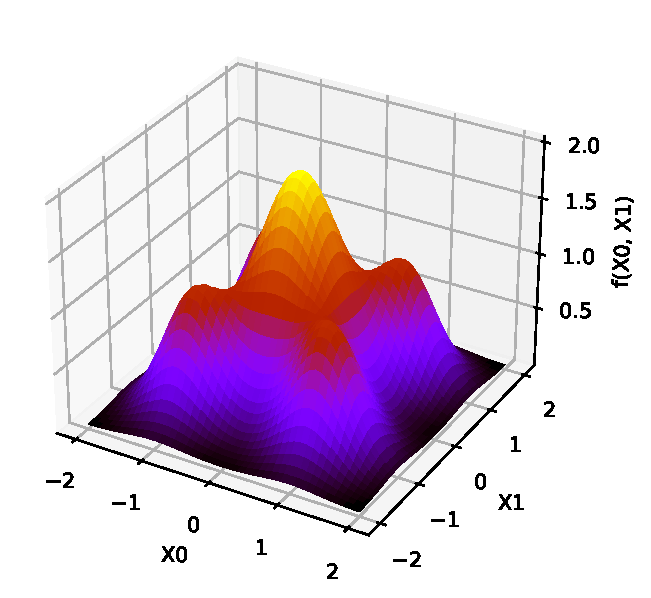
\includegraphics[width=0.69\textwidth]{../../code/testbed/pde0A/sol_pde_0a.pdf}
	}
	\unterschrift{PDE 0A Gauss Kernel solution plot}{}{}
	\label{fig:sol_plot_0A}
\end{figure}





\underline{\textbf{PDE 0B: GSin Kernel}}

\underline{Problem PDE:} 
\begin{equation}
\label{eq:pde0b}
\begin{split}
\frac{\partial^2 u}{\partial x^2} + \frac{\partial^2 u}{\partial y^2} = \\
2 e^{-2   (x^2 + y^2)} (2   sin(-2   (x^2 + y^2)) + 2   (1-8   x^2) cos(-2   (x^2 + y^2))) + \\
2 e^{-2   (x^2 + y^2)} (2   sin(-2   (x^2 + y^2)) + 2   (1-8   y^2) cos(-2   (x^2 + y^2))) + \\
2 e^{-1   (x^2 + y^2)} (1   sin(-1   (x^2 + y^2)) + 1   (1-4   x^2) cos(-1   (x^2 + y^2))) + \\
2 e^{-1   (x^2 + y^2)} (1   sin(-1   (x^2 + y^2)) + 1   (1-4   y^2) cos(-1   (x^2 + y^2))) + \\
2 e^{-0.1 (x^2 + y^2)} (0.1 sin(-0.1 (x^2 + y^2)) + 0.1 (1-0.4 x^2) cos(-0.1 (x^2 + y^2))) + \\
2 e^{-0.1 (x^2 + y^2)} (0.1 sin(-0.1 (x^2 + y^2)) + 0.1 (1-0.4 y^2) cos(-0.1 (x^2 + y^2))) \\
\text{on the domain } \Omega : x, y \in [-2,2] \\
\text{subjected to: } \\
u(x,2) =	 e^{-2  (x^2 + 4  )}  sin(2  ((x^2 + 4  ))) + e^{-1  (x^2 + 4  )}  sin(1  ((x^2 + 4  ))) + e^{-0.1(x^2 + 4  )}  sin(0.1((x^2 + 4  ))) \\				u(x,-2)= 	 e^{-2  (x^2 + 4  )}  sin(2  ((x^2 + 4  ))) + e^{-1  (x^2 + 4  )}  sin(1  ((x^2 + 4  ))) + e^{-0.1(x^2 + 4  )}  sin(0.1((x^2 + 4  ))) \\				u(2,y) = 	 e^{-2  (4   + y^2)}  sin(2  ((4   + y^2))) + e^{-1  (4   + y^2)}  sin(1  ((4   + y^2))) + e^{-0.1(4   + y^2)}  sin(0.1((4   + y^2))) \\
u(-2,y)= 	 e^{-2  (4   + y^2)}  sin(2  ((4   + y^2))) + e^{-1  (4   + y^2)}  sin(1  ((4   + y^2))) + e^{-0.1(4   + y^2)}  sin(0.1((4   + y^2))) \\
\end{split}
\end{equation}

\newpage

\underline{Solution:}
\begin{equation}
\label{eq:sol0B}
\begin{split}
u_{ext}(x,y) = & e^{-2  (x^2 + y^2)}  sin(2  ((x^2 + y^2))) \\
 			   & e^{-1  (x^2 + y^2)}  sin(1  ((x^2 + y^2))) \\
 			   & e^{-0.1(x^2 + y^2)}  sin(0.1((x^2 + y^2))) \\
\end{split}
\end{equation}


\begin{figure}[H]
	\centering
	\noindent\adjustbox{max width=\linewidth}{
		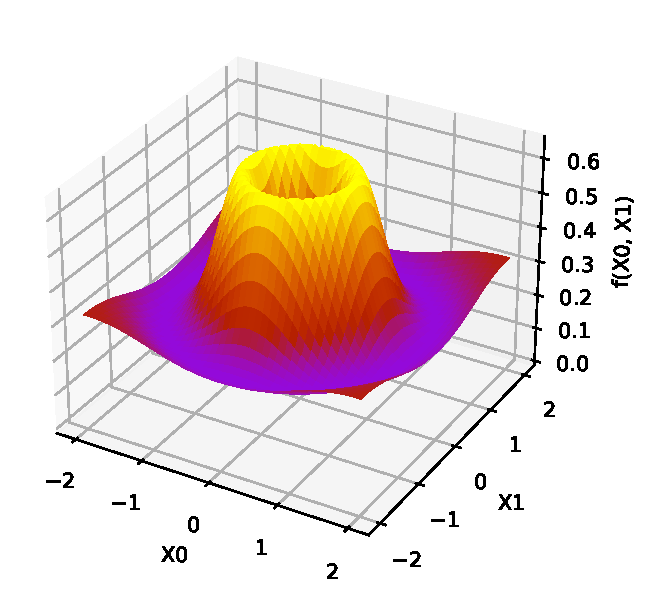
\includegraphics[width=0.69\textwidth]{../../code/testbed/pde0B/sol_pde_0b.pdf}
	}
	\unterschrift{PDE 0B Gsin Kernel solution plot}{}{}
	\label{fig:sol_plot_0B}
\end{figure}



\newpage


\underline{\textbf{PDE 1: Polynomial 2D}} 

\underline{Problem PDE:} 
\begin{equation}
\label{eq:pde1}
\begin{split}
-\frac{\partial^2 u}{\partial x^2} - \frac{\partial^2 u}{\partial y^2} = \\
-2^{40}y^{10}(1-y)^{10}[90x^8(1-x)^{10} -200x^9(1-x)^9 + 90x^{10}(1-x)^8] \\
-2^{40}x^{10}(1-x)^{10}[90y^8(1-y)^{10} -200y^9(1-y)^9 + 90y^{10}(1-y)^8] \\
\text{on the domain } \Omega: x,y \in [0,1] \\
\text{subjected to: } \\
u(x,1) = 0 \\
u(x,0) = 0 \\
u(1,y) = 0 \\
u(0,y) = 0 \\
\end{split}
\end{equation}


\underline{Solution:} 
\begin{equation}
\label{eq:sol1}
u_{ext}(x,y) = 2^{40}x^{10}(1-x)^{10}y^{10}(1-y)^{10}
\end{equation}


\begin{figure}[H]
	\centering
	\noindent\adjustbox{max width=\linewidth}{
		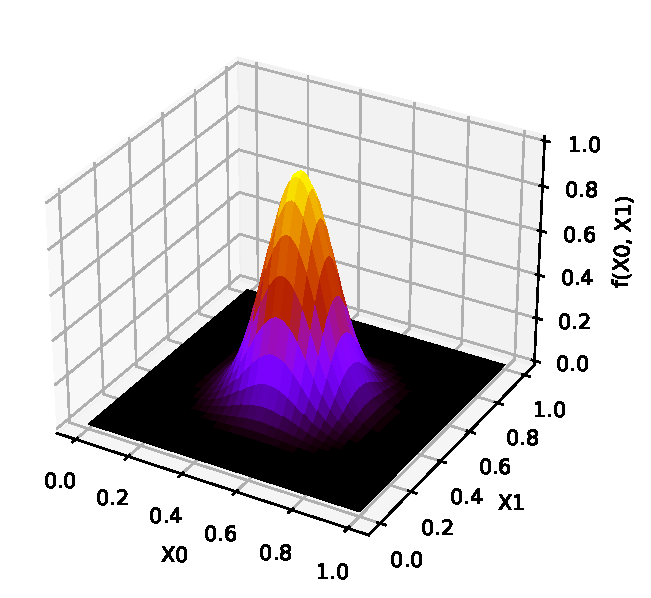
\includegraphics[width=0.69\textwidth]{../../code/testbed/pde1/sol_pde_1.pdf}
	}
	\unterschrift{PDE 1 Polynomial 2D solution plot}{}{}
	\label{fig:sol_plot_1}
\end{figure}



\newpage


\underline{\textbf{PDE 2: Chaquet PDE 1}}

\underline{Problem PDE:} 
\begin{equation}
\label{eq:pde2}
\begin{split}
\frac{\partial^2 u}{\partial x^2} + \frac{\partial^2 u}{\partial y^2} = e^{-x} (x-2 + y^3 + 6y) \\
\text{on the domain } \Omega: \mathbf{x} \in [0,1] \\
\text{subjected to: } \\
u(x,0) = xe^{-x}
u(x,1) = (x + 1)e^{-x}
u(0,y) = y^3 \\
u(1,y) = (1 + y^3) e^{-1}
\end{split}
\end{equation}


\underline{Solution:}
\begin{equation}
\label{eq:sol2}
u_{ext}(x,y) = (x + y^3) e^{-x}
\end{equation}



\begin{figure}[H]
	\centering
	\noindent\adjustbox{max width=\linewidth}{
		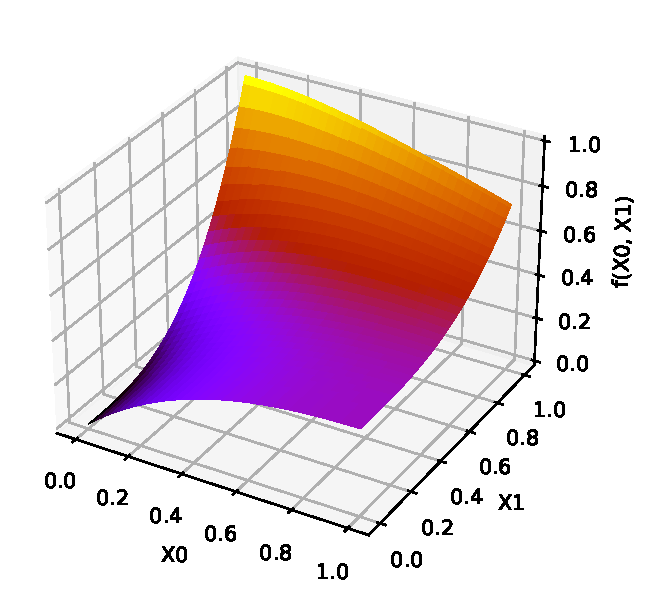
\includegraphics[width=0.69\textwidth]{../../code/testbed/pde2/sol_pde_2.pdf}
	}
	\unterschrift{PDE 2 Chaquet PDE 1 solution plot}{}{}
	\label{fig:sol_plot_2}
\end{figure}




\newpage



\underline{\textbf{PDE 3: Chaquet PDE 3}}

\underline{Problem PDE:} 
\begin{equation}
\label{eq:pde3}
\begin{split}
\frac{\partial^2 u}{\partial x^2} + \frac{\partial^2 u}{\partial y^2} = 4 \\
\text{on the domain } \Omega: \mathbf{x} \in [0,1] \\
\text{subjected to: } \\
u(x,0) = x^2 + x + 1 \\
u(x,1) = x^2 + x + 3 \\
u(1,y) = y^2 + y + 3 \\
u(0,y) = y^2 + y + 1 \\
\end{split}
\end{equation}


\underline{Solution}
\begin{equation}
\label{eq:sol3}
u_{ext}(x,y) = x^2 + y^2 + x + y + 1
\end{equation}


\begin{figure}[H]
	\centering
	\noindent\adjustbox{max width=\linewidth}{
		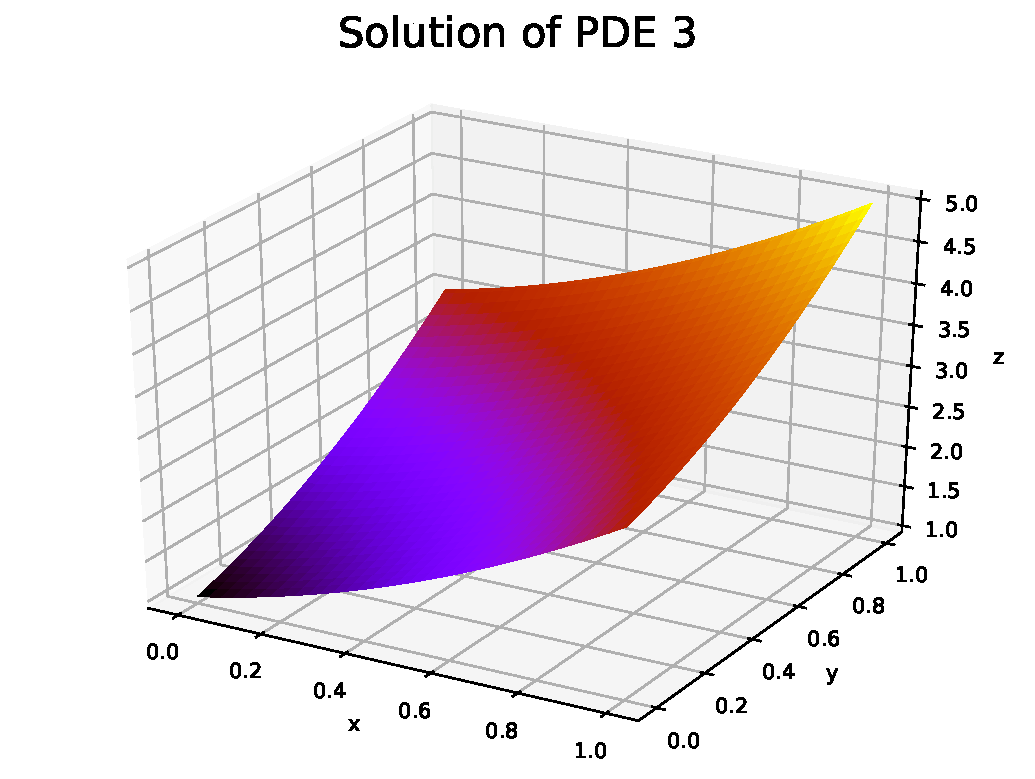
\includegraphics[width=0.69\textwidth]{../../code/testbed/pde3/sol_pde_3.pdf}
	}
	\unterschrift{PDE 3 Chaquet PDE 3 solution plot}{}{}
	\label{fig:sol_plot_3}
\end{figure}



\newpage




\underline{\textbf{PDE 4: Sine Bump 2D}} 

\underline{Problem PDE:}
\begin{equation}
\label{eq:pde4}
\begin{split}
-\frac{\partial^2 u}{\partial x^2} - \frac{\partial^2 u}{\partial y^2} = 2\pi^2 sin(\pi x) sin(\pi y) \\
\text{on the domain } \Omega: \mathbf{x} \in [0,1] \\
\text{subjected to: } \\
u(x,0) = 0 \\
u(x,1) = 0 \\
u(0,y) = 0 \\
u(1,y) = 0 \\
\end{split}
\end{equation}


\underline{Solution:}
\begin{equation}
\label{eq:sol4}
u_{ext}(x,y) = sin(\pi x)sin(\pi y)
\end{equation}



\begin{figure}[H]
	\centering
	\noindent\adjustbox{max width=\linewidth}{
		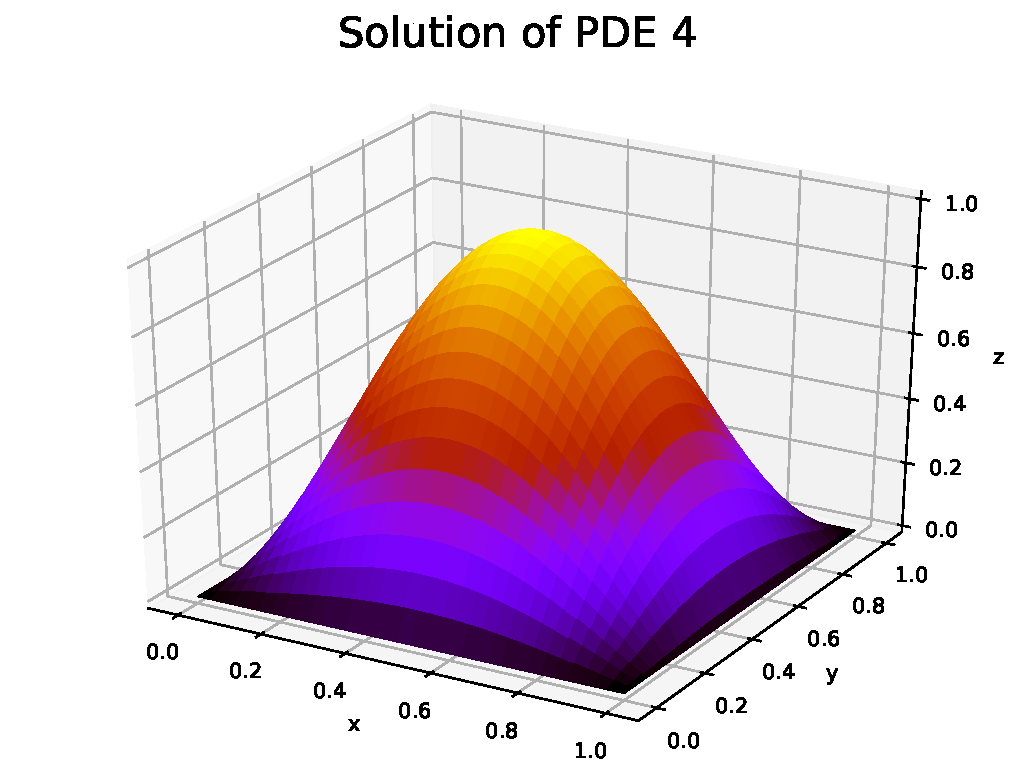
\includegraphics[width=0.69\textwidth]{../../code/testbed/pde4/sol_pde_4.pdf}
	}
	\unterschrift{PDE 4 Sine Bump 2D solution plot}{}{}
	\label{fig:sol_plot_4}
\end{figure}




\newpage







\underline{\textbf{PDE 5: Arctan Circular Wave Front}} 

\underline{Problem PDE:}
\begin{equation}
\label{eq:pde5}
\begin{split}
-\frac{\partial^2 u}{\partial x^2} - \frac{\partial^2 u}{\partial y^2} = \frac{16000(\sqrt{(x - 0.05)^2 + (y - 0.05)^2} -0.7)}{(1 + 400 (-0.7 + \sqrt{(x - 0.05)^2 + (y - 0.05)^2})^2)^2} \\
+ \frac{20 (x - 0.05)^2 + 20 (y - 0.05)^2}{(1 + 400 (\sqrt{(x - 0.05)^2 + (y - 0.05)^2} -0.7)^2) ((x - 0.05)^2 + (y - 0.05)^2)^{3/2}} \\
- \frac{40}{(1 + 400 (\sqrt{(y - 0.05)^2 + (x - 0.05)^2} -0.7)^2) \sqrt{(y - 0.05)^2 + (x - 0.05)^2}} \\
\text{on the domain } \Omega: \mathbf{x} \in [0,1] \\
\text{subjected to: } \\
u(x,0) = tan^{-1}\left(20 \left(\sqrt{(x-0.05)^2 + 0.0025} -0.7\right)\right) \\
u(x,1) = tan^{-1}\left(20 \left(\sqrt{(x-0.05)^2 + 0.9025} -0.7\right)\right) \\
u(0,y) = tan^{-1}\left(20 \left(\sqrt{0.0025 + (y-0.05)^2} -0.7\right)\right) \\
u(1,y) = tan^{-1}\left(20 \left(\sqrt{0.9025 + (y-0.05)^2} -0.7\right)\right) \\
\end{split}
\end{equation}

\underline{Solution:}
\begin{equation}
\label{eq:sol5}
u_{ext}(x,y) = tan^{-1}\left(20 \left(\sqrt{(x-0.05)^2 + (y-0.05)^2} -0.7\right)\right)
\end{equation}



\begin{figure}[H]
	\centering
	\noindent\adjustbox{max width=\linewidth}{
		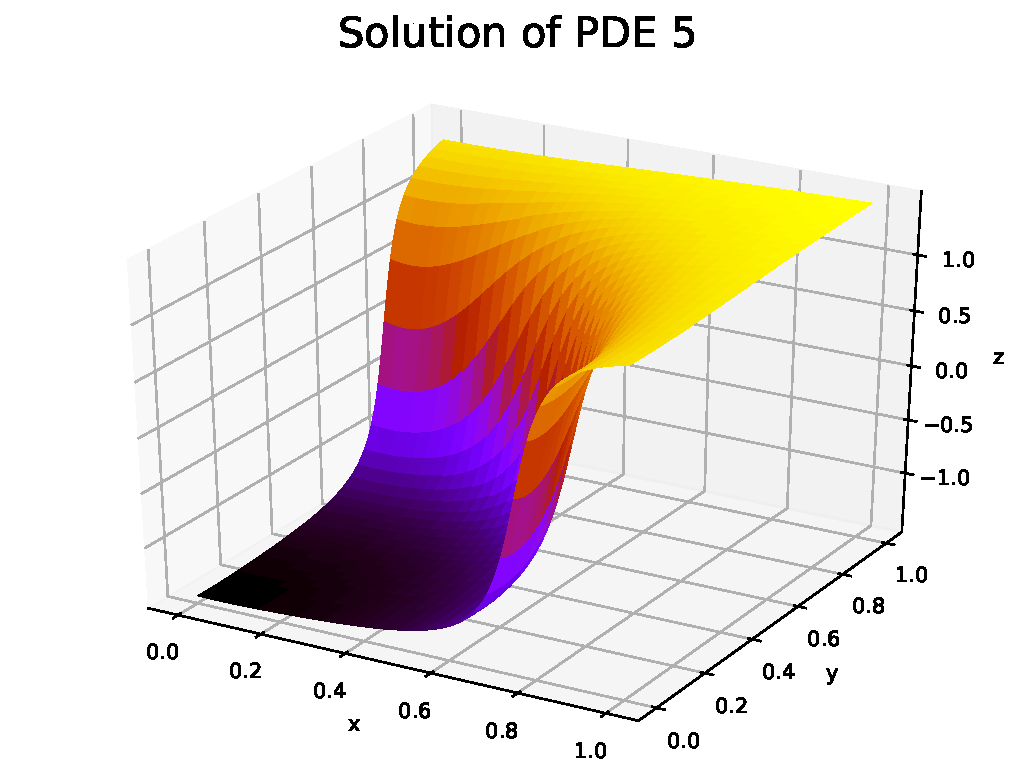
\includegraphics[width=0.69\textwidth]{../../code/testbed/pde5/sol_pde_5.pdf}
	}
	\unterschrift{PDE 5 Arctan Circular Wave Front solution plot}{}{}
	\label{fig:sol_plot_5}
\end{figure}




\newpage




\underline{\textbf{PDE 6: Peak 2D}} 

\underline{Problem PDE:}
\begin{equation}
\label{eq:pde6}
\begin{split}
-\frac{\partial^2 u}{\partial x^2} - \frac{\partial^2 u}{\partial y^2} = \\
-(4 \cdot 10^6 x^2 -4 \cdot 10^6 x + 998 \cdot 10^3)e^{-1000((x-0.5)^2 + (y-0.5)^2)} \\
-(4 \cdot 10^6 y^2 -4 \cdot 10^6 y + 998 \cdot 10^3)e^{-1000((x-0.5)^2 + (y-0.5)^2)} \\
\text{on the domain } \Omega: \mathbf{x} \in [0,1] \\
\text{subjected to: } \\
u(x,0) = e^{-1000((x-0.5)^{2} + 0.25)} \\
u(x,1) = e^{-1000((x-0.5)^{2} + 0.25)} \\
u(0,y) = e^{-1000(0.25 + (y-0.5)^{2})} \\
u(1,y) = e^{-1000(0.25 + (y-0.5)^{2})} \\
\end{split}
\end{equation}

\underline{Solution:}
\begin{equation}
\label{eq:sol6}
u_{ext}(x,y) = e^{-1000((x-0.5)^{2} + (y-0.5)^{2})}
\end{equation}




\begin{figure}[H]
	\centering
	\noindent\adjustbox{max width=\linewidth}{
		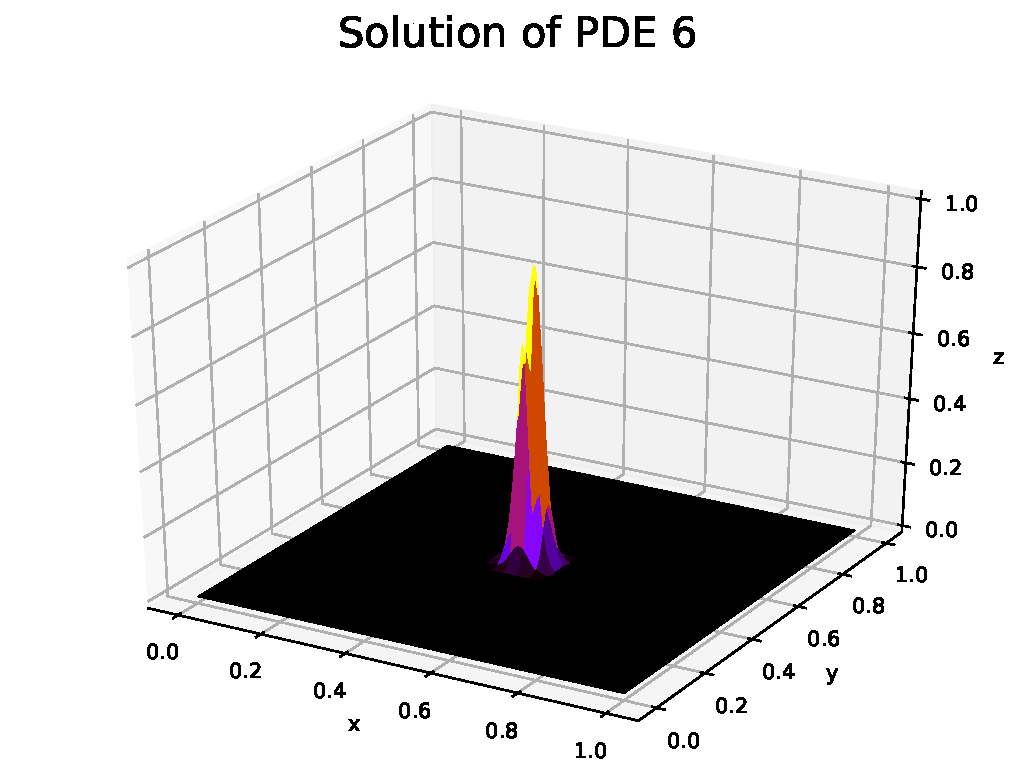
\includegraphics[width=0.69\textwidth]{../../code/testbed/pde6/sol_pde_6.pdf}
	}
	\unterschrift{PDE 6 Peak 2D solution plot}{}{}
	\label{fig:sol_plot_6}
\end{figure}




\newpage





\underline{\textbf{PDE 7: Boundary Line Singularity}} 

\underline{Problem PDE:} 
\begin{equation}
\label{eq:pde7}
\begin{split}
-\frac{\partial^2 u}{\partial x^2} - \frac{\partial^2 u}{\partial y^2} = 0.24 x^{-1.4}\\
\text{on the domain } \Omega: \mathbf{x} \in [0,1] \\
\text{subjected to: } \\
u(x,0) = x^{0.6} \\
u(x,1) = x^{0.6} \\
u(0,y) = 0 \\
u(1,y) = 1^{0.6} \\
\end{split}
\end{equation}


\underline{Solution:} 
\begin{equation}
\label{eq:sol7}
u_{ext}(x,y) = x^{0.6}
\end{equation}



\begin{figure}[H]
	\centering
	\noindent\adjustbox{max width=\linewidth}{
		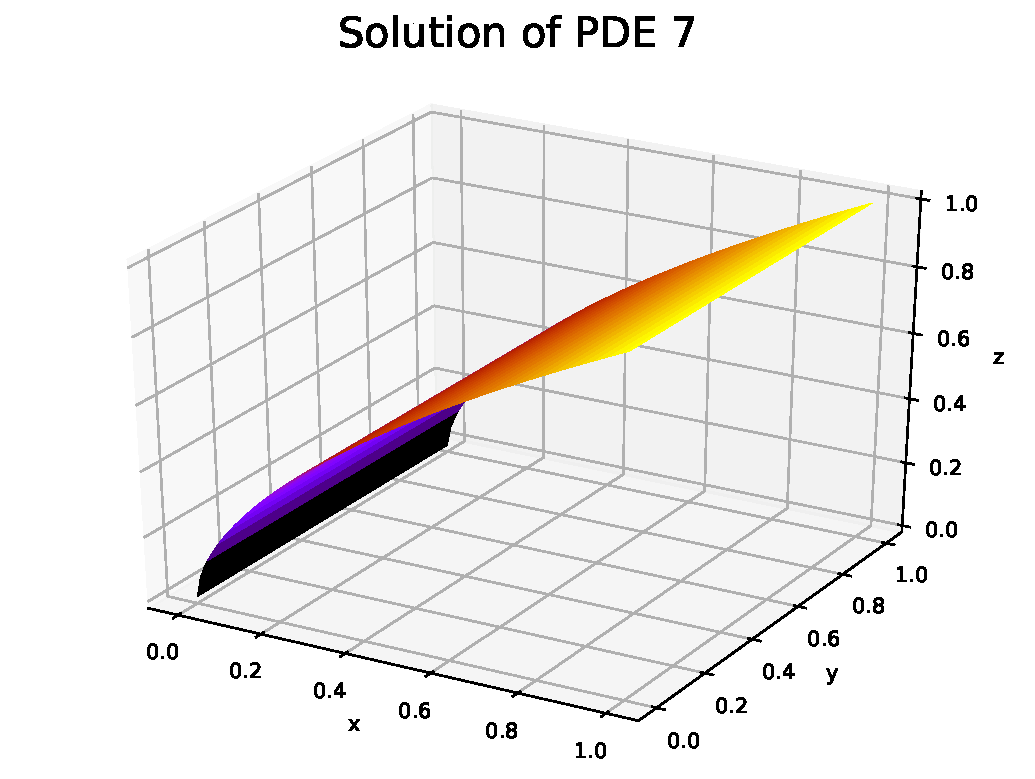
\includegraphics[width=0.69\textwidth]{../../code/testbed/pde7/sol_pde_7.pdf}
	}
	\unterschrift{PDE 7 Boundary Line Singularity solution plot}{}{}
	\label{fig:sol_plot_7}
\end{figure}




\newpage





\underline{\textbf{PDE 8: Interior Point Singularity}} 

\underline{Problem PDE:} 
\begin{equation}
\label{eq:pde8}
\begin{split}
\frac{\partial^2 u}{\partial x^2} + \frac{\partial^2 u}{\partial y^2} = \frac{1}{\sqrt{x^2 - x + y^2 - y + 0.5}} \\
\Omega: \mathbf{x} \in [0,1] \\
\text{on the domain } \text{subjected to: } \\
u(x,0) = \sqrt{(x-0.5)^2 + 0.25} \\
u(x,1) =  \sqrt{(x-0.5)^2 + 0.25} \\
u(0,y) = \sqrt{0.25 + (y-0.5)^2} \\
u(1,y) =  \sqrt{0.25 + (y-0.5)^2} \\
\end{split}
\end{equation}

\underline{Solution:}
\begin{equation}
\label{eq:sol8}
u_{ext}(x,y) = \sqrt{(x-0.5)^2 + (y-0.5)^2}
\end{equation}


\begin{figure}[H]
	\centering
	\noindent\adjustbox{max width=\linewidth}{
		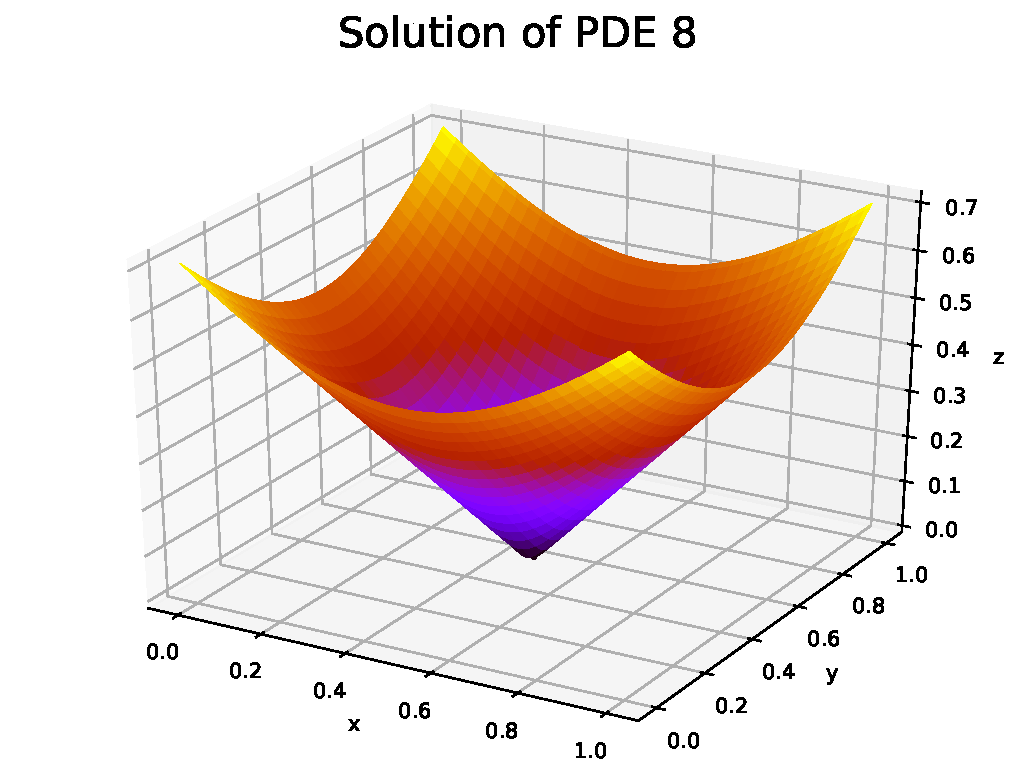
\includegraphics[width=0.69\textwidth]{../../code/testbed/pde8/sol_pde_8.pdf}
	}
	\unterschrift{PDE 8 Interior Point Singularity solution plot}{}{}
	\label{fig:sol_plot_8}
\end{figure}





\newpage




\underline{\textbf{PDE 9: Arctan Wave Front Homogeneous Boundary Conditions 2D}} 

\underline{Problem PDE:}
\begin{equation}
\label{eq:pde9}
\begin{split}
-\frac{\partial^2 u}{\partial x^2} - \frac{\partial^2 u}{\partial y^2} = \\
\frac{20\sqrt{2}(x^2 + y^2 -2x^2y - 2xy^2 + 4xy - x - y)}{400(\frac{x+y}{\sqrt{2}}-0.8)^2+1} \\
+\frac{16000(1-x)x(1-y)y(\frac{x+y}{\sqrt{2}}-0.8)}{(400(\frac{x+y}{\sqrt{2}}-0.8)^2+1)^2} \\
+ tan^{-1}\left(20\left(\frac{x+y}{\sqrt{2}}-0.8\right)\right)(2(1-y)y + 2(1-x)x)  \\
\text{on the domain } \Omega: \mathbf{x} \in [0,1] \\
\text{subjected to: } \\
u(x,0) = 0 \\
u(x,1) = 0 \\
u(0,y) = 0 \\
u(1,y) = 0 \\
\end{split}
\end{equation}


\underline{Solution:}
\begin{equation}
\label{eq:sol9}
u_{ext}(x,y) = tan^{-1}\left(20\left(\frac{(x + y)}{\sqrt{2}} -0.8\right)\right)x(1-x)y(1-y)
\end{equation}



\begin{figure}[H]
	\centering
	\noindent\adjustbox{max width=\linewidth}{
		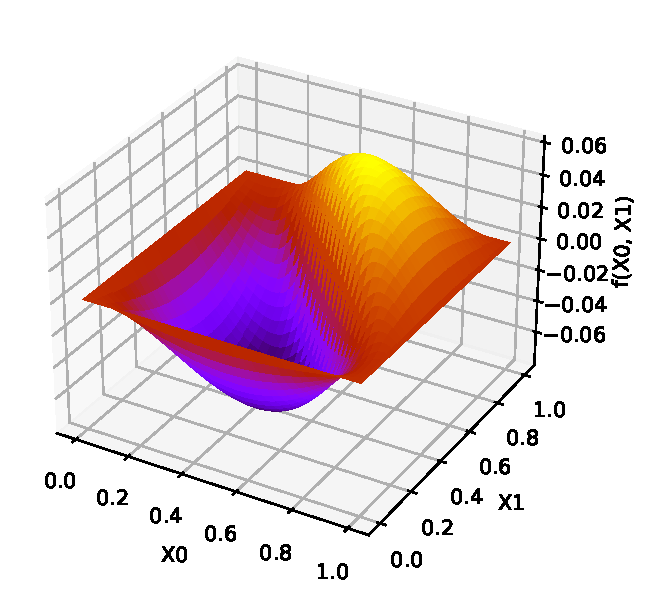
\includegraphics[width=0.65\textwidth]{../../code/testbed/pde9/sol_pde_9.pdf}
	}
	\unterschrift{PDE 9 Arctan Wave Front Homogeneous Boundary Conditions 2D solution plot}{}{}
	\label{fig:sol_plot_9}
\end{figure}





\chapter{Software Architecture}
\label{chap:software_architecture}

\begin{figure}[H]
	\centering
	\noindent\adjustbox{max width=\linewidth}{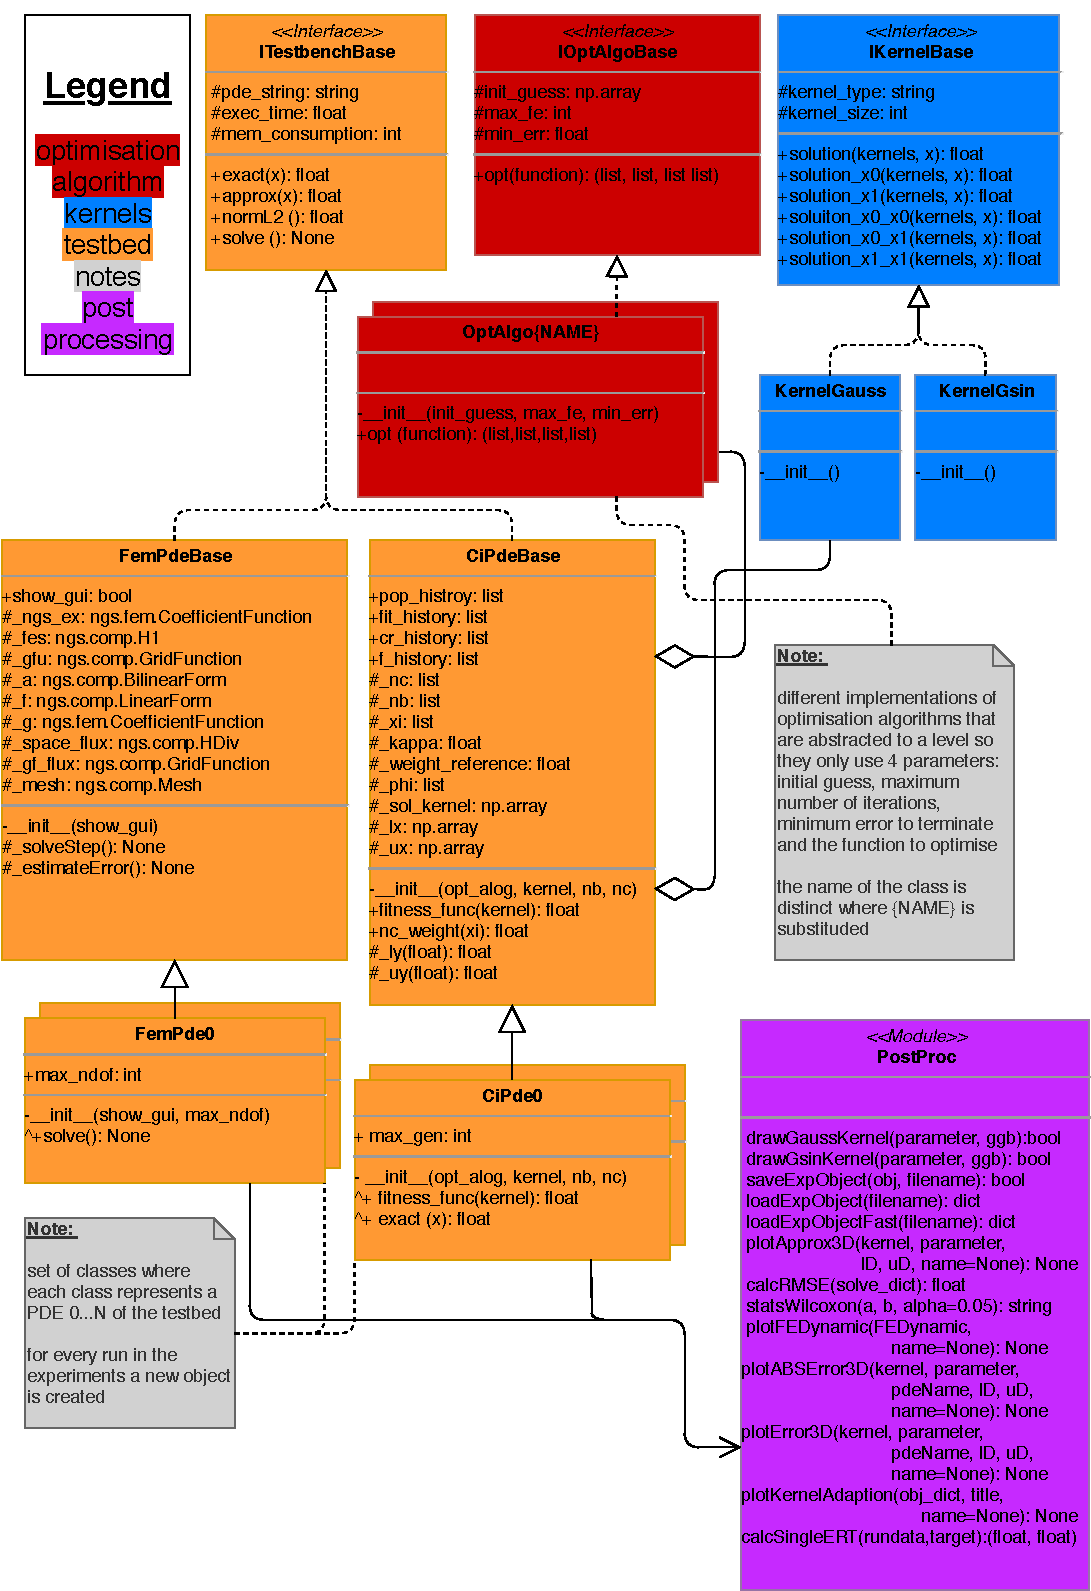
\includegraphics[width=1\textwidth]{../../code/uml_diag/testbench_uml_class.pdf}
	}
	\unterschrift{This \gls{uml} class diagram describes the software architecture defined to prepare, run and evaluate the experiments. }{}{}
	\label{fig:software_architecture}
\end{figure}

\chapter{solve function}
\label{chap:solve_function}

\begin{algorithm}[H]
	\SetAlgoNoLine
	\DontPrintSemicolon
	\SetKwFunction{Fsolve}{solve}
	\SetKwProg{Fn}{Function}{:}{}
	\Fn{\Fsolve{}}{
		$gc.disable()$\;
		\While{$gc.isenabled()$} {
			$time.sleep(0.1)$\;
		}	
		$process = psutil.Process()$\;
		$memstart = process.memory\text{\textunderscore}info().rss$\;
		$t\text{\textunderscore}start = time.time()$\;
		\tcp{perform solver steps}
		\tcp{that are particular}
		\tcp{to FEM or CI solver}
		$self.\text{\textunderscore}exec\text{\textunderscore}time = time.time() - t\text{\textunderscore}{start}$\;
		$memstop = process.memory\text{\textunderscore}info().rss - memstart$\;
		$gc.enable()$\;
		$gc.collect()$\;
	}
	\unterschrift{solve function pseudocode}{}{}
	\label{algo: solve}
\end{algorithm}

\end{document}